\section{Results}
\textit{- Present your \textbf{findings} in a logical and coherent manner.}

This section presents the main results of the FRESNEL field campaign, focusing on the integration of model forecasts, target sampling, and data assimilation using autonomous underwater vehicles (AUVs). The analysis combines CMEMS and statistical model forecasts (as described in the Methods section) with in situ observations to assess how the proposed data-cycle approach can enhance short-term ocean prediction in a dynamic coastal environment.

Figure \figure{sst} provides an overview of the environmental conditions observed during the three-day experimental window considered in this study (29–31 October). The background fields correspond to the Level-3 Sea Surface Temperature (SST) product from the E.U. Copernicus Marine Service Information (url{DOI:10.48670/moi-00310})


\begin{itemize}
    \item Environmental context
    
\begin{figure}
    \centering
    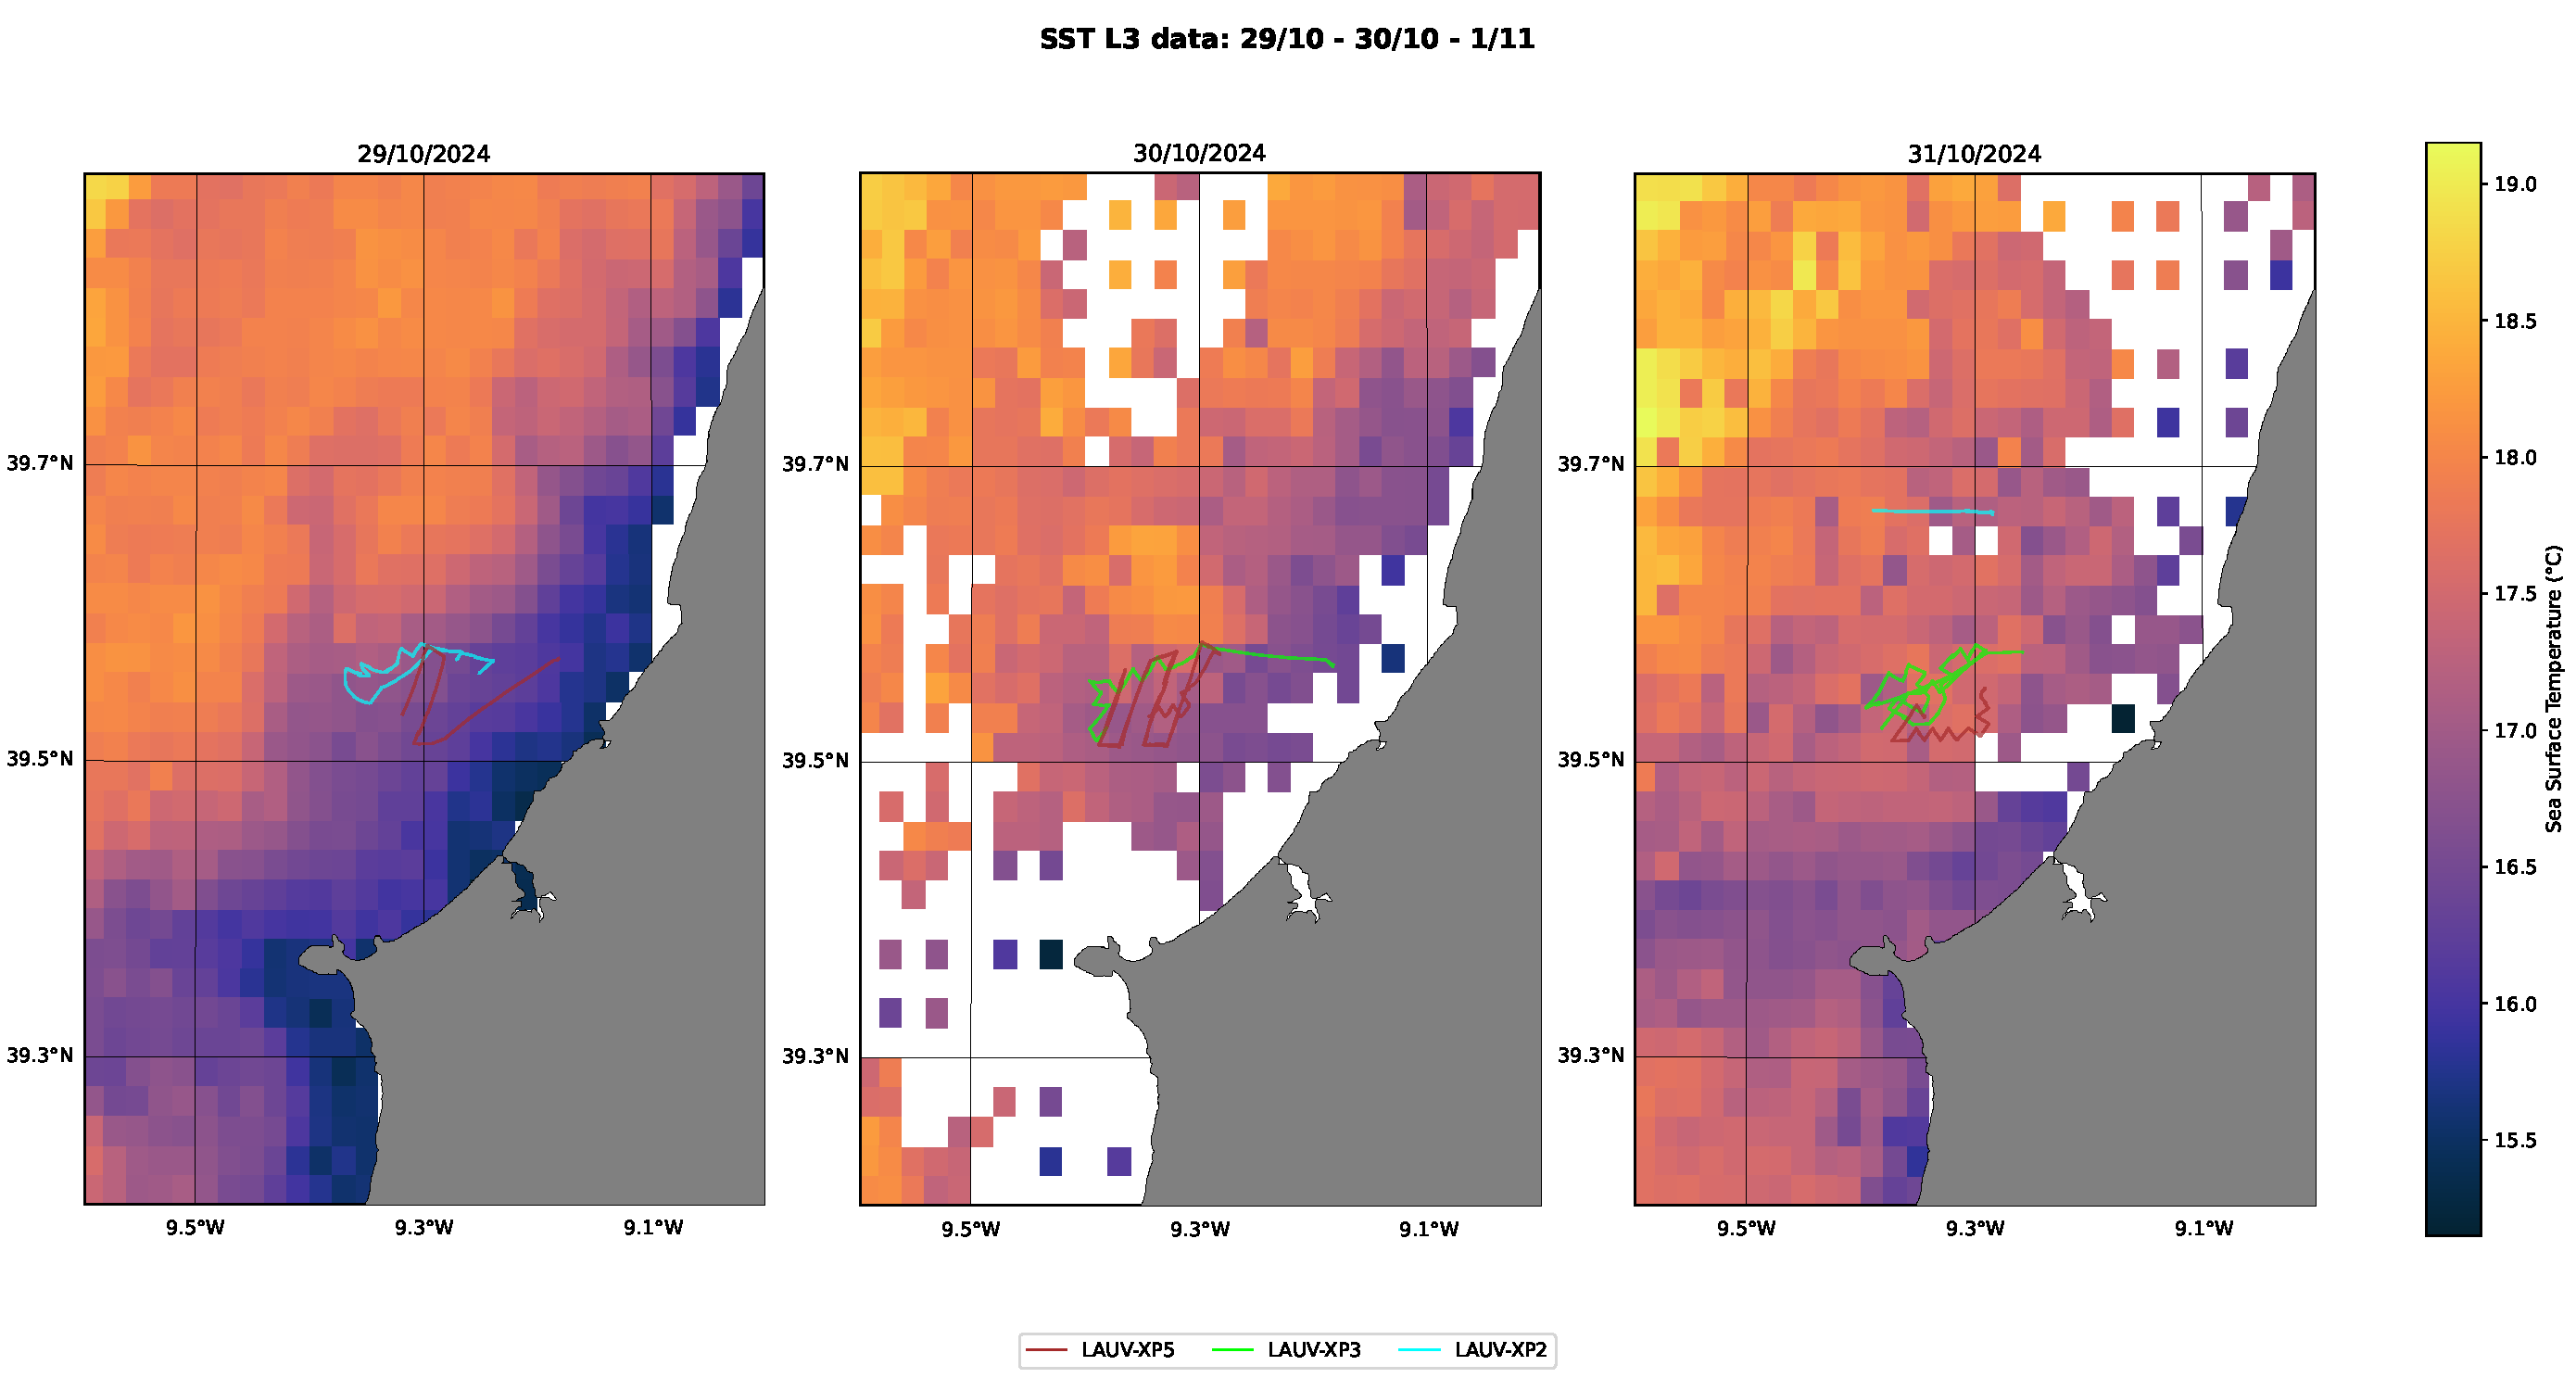
\includegraphics[width=1\linewidth]{fig/SST_L3_color1.pdf}
    \caption{L3 SST data + AUV trajectories over 3 days}
    \label{fig:sst}
\end{figure}

\begin{figure}
    \centering
    \includegraphics[width=1\linewidth]{fig/Figure2_100m.pdf}
    \caption{temperature data collected by AUV in depth (yy) over time (xx)}
    \label{fig:temperatureprofiles}
\end{figure}
    
    
    \item RMS table (all cases) + rms figure (just A+D cases)
\end{itemize}

 
\textit{- Use \textbf{subheadings} to organize different experiments or analyses.}
